% Notes and solutions


% -------------------------------------------------
% Package imports
% -------------------------------------------------
\documentclass[12pt, a4paper]{article}
\usepackage[utf8]{inputenc}% Input encoding
\usepackage[english]{babel}% Set language to english
\usepackage{graphicx}% For importing graphics
\usepackage{amsthm, amsfonts, amssymb, bm}% All the AMS packages
\usepackage{mathtools}% Fixes a few AMS bugs
\usepackage[expansion=false]{microtype}% Fixes to make typography better
\usepackage{hyperref}% For \href{URL}{text}
\usepackage{fancyhdr}% For fancy headers
\usepackage[sharp]{easylist}% Easy nested lists
\usepackage{parskip}% Web-like paragraphs
\usepackage{multicol}% For multiple columns
\usepackage{tikz-cd}% For diagrams
\usepackage{microtype}
\usepackage{listings}% To include source-code
\usepackage[margin = 2.5cm, includehead]{geometry}% May be used to set margins
\usepackage{nicefrac}% Enables \nicefrac{nom}{denom}
%\usepackage[sc]{mathpazo}% A nice font, alternative to CM
\usepackage{booktabs}

% -------------------------------------------------
% Package setup
% -------------------------------------------------

\newcommand{\Title}{Learning Machine Learning}
\newcommand{\Subtitle}{A summary of main ideas and concepts}
\newcommand{\Author}{tommyod}
\newcommand{\listSpace}{-0.5em}% Global list space

\title{\Title}
\author{\Author}

% Shortcuts for sets and other stuff in mathematics
\newcommand{\Q}{\mathbb{Q}}
\newcommand{\R}{\mathbb{R}}
\newcommand{\C}{\mathbb{C}}
\newcommand{\D}{\mathcal{D}}
\newcommand{\Reg}{\mathcal{R}}
\newcommand{\Class}{\mathcal{C}}
\newcommand{\Z}{\mathbb{Z}}
\renewcommand{\sf}[1]{\mathsf{#1}}
\newcommand{\vect}[1]{\bm{#1}}
\newcommand{\norm}[1]{\left\lVert#1\right\rVert}
\newcommand{\abs}[1]{\left\lvert#1\right\rvert}

% Shortcuts for probability distributions
\DeclareMathOperator{\N}{\mathcal{N}}
\DeclareMathOperator{\Bern}{\operatorname{Bern}}
\DeclareMathOperator{\Beta}{\operatorname{Beta}}
\DeclareMathOperator{\Bin}{\operatorname{Bin}}
\DeclareMathOperator{\St}{\operatorname{St}}
\DeclareMathOperator{\U}{\operatorname{U}}
\DeclareMathOperator{\KL}{\operatorname{KL}}

% Shortcuts for statistical operators
\DeclareMathOperator{\E}{\mathbb{E}}
\DeclareMathOperator{\var}{\operatorname{var}}
\DeclareMathOperator{\cov}{\operatorname{cov}}
\DeclareMathOperator{\SD}{\operatorname{SD}}
\renewcommand{\H}{\operatorname{H}}



% Change the section command to inluce lines, save space, etc.
%\usepackage{titlesec}
%\titlespacing\subsection{0pt}{6pt plus 4pt minus 2pt}{-0.8em plus 4pt minus 2pt}
%\titlespacing\paragraph{0pt}{6pt plus 4pt minus 2pt}{8pt plus 4pt minus 2pt}
%\titleformat{\section}
%{\normalfont\Large\bfseries}{\thesection}{0em}{$\vartriangleright$ }[{\titlerule[1.2pt]}]

% -------------------------------------------------
% Document start
% -------------------------------------------------
\begin{document}
	
\maketitle
\begin{abstract}
This document contains some notes and solutions to the book ``Pattern Classification'' by Duda et al.
\end{abstract}

\tableofcontents

\section{Notes from ``Pattern Recognition''}

\section{Solutions to ``Pattern Recognition''}

\subsection{Bayesian Decision Theory}

\subsubsection*{Problem 2.6}
\begin{easylist}[enumerate]
\ListProperties(Space=\listSpace, Space*=\listSpace, Numbers1=l, FinalMark1={)})
# We want the probability of choosing action $\alpha_2$ to be smaller than, or equal to, $E_1$, given that the true state of nature is $\omega_1$.
Let's assume that $\mu_1 < \mu_2$ and that the decision threshold is $x^*$, so we decide $\alpha_2$ if $x > x^*$.
We then have
\begin{align*}
	P(\alpha_2 | \omega_1) &\leq E_1 \\
	p(x > x^* | \omega_1) &\leq E_1 \\
	\left[1 - \int_{0}^{x^*} p(x | \omega_1)  \, dx \right] &\leq E_1
\end{align*}
We let $\Phi: \R \to \left[0, 1\right]$ denote the cumulative Gaussian distribution, and $\Phi^{-1}: \left[0, 1\right] \to \R$ it's inverse function.
Making use of $\Phi$ we write
\begin{align*}
1 - \Phi \left( \frac{x^* - \mu_1}{\sigma_1} \right) &\leq E_1 \\
x^* \geq \mu_1 + \sigma_1 \Phi^{-1} \left(1 - E_1 \right).
\end{align*}
If the desired error is close to zero, then $x^*$ goes to positive infinity.
If the desired error is close to one, then $x^*$ goes to negative infinity.

# The error rate for classifying $\omega_2$ as $\omega_1$ is
\begin{equation*}
	P(\alpha_1 | \omega_2) = 	p(x \leq x^* | \omega_2) = \int_{0}^{x^*} p(x| \omega_2) \, dx 
	= 
	\Phi \left(  \frac{x^* - \mu_2}{\sigma_2}  \right).
\end{equation*}
Making use of $x^*$ from the previous problem, we obtain
\begin{equation*}
 \Phi \left(  \frac{ \mu_1 + \sigma_1 \Phi^{-1} \left(1 - E_1 \right) - \mu_2}{\sigma_2}  \right) 
 =
\Phi \left(  \frac{\mu_1 - \mu_2}{\sigma_2} + \frac{\sigma_1}{\sigma_2}  \Phi^{-1} \left(1 - E_1 \right) \right).
\end{equation*}
# The overall error rate becomes
\begin{align*}
	P(\text{error}) &= P(\alpha_1, \omega_2) + P(\alpha_2, \omega_1) \\
	&= P(\alpha_1 | \omega_2) P(\omega_2) + P(\alpha_2| \omega_1) P(\omega_1) \\
	&= \frac{1}{2} \left[  P(\alpha_1 | \omega_2) +  P(\alpha_2| \omega_1) \right] \\
	&= \frac{1}{2} \left[ E_1 +  \Phi \left(  \frac{\mu_1 - \mu_2}{\sigma_2} + \frac{\sigma_1}{\sigma_2}  \Phi^{-1} \left(1 - E_1 \right) \right) \right].
\end{align*}
In the last equality we used the results from the previous problems.

# We substitute the given values into the equations, and obtain $x^* \approx 0.6449$. The total error rate is $P(\text{error}) \approx 0.2056$.
# The Bayes error rate, as a function of $x^*$, is given by
\begin{align*}
	P(\text{error}) = P(\alpha_2 | \omega_1) P(\omega_1) + P(\alpha_1| \omega_2) P(\omega_2) \\
	= \frac{1}{2} \left[ p( x > x^*| \omega_1)  + p( x < x^* | \omega_2) \right]   \\
	= \frac{1}{2} \left[ \left( 1 - \Phi \left( \frac{x^* - \mu_1}{\sigma_1}\right)\right) +  \Phi \left( \frac{x^* - \mu_2}{\sigma_2}\right)  \right]
\end{align*}
The Bayes error rate is depicted in Figure \ref{fig:duda_ch2_prob6}.

\begin{figure}[ht!]
\centering
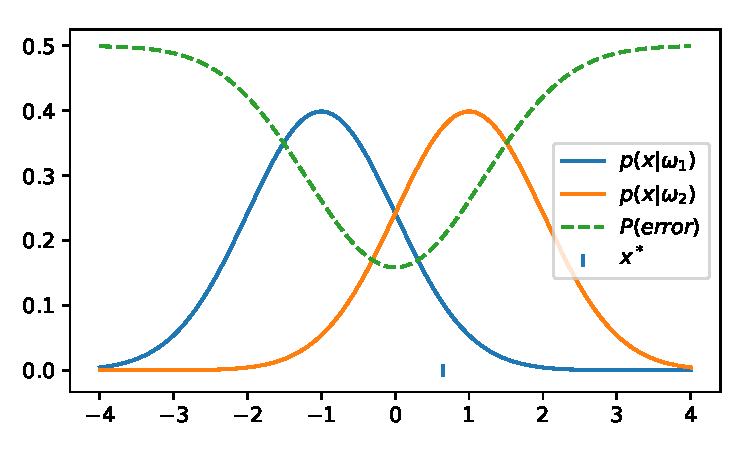
\includegraphics[width=0.5\linewidth]{figs/duda_ch2_prob6}
\caption{Graf accompanying problem 2.6.}
\label{fig:duda_ch2_prob6}
\end{figure}


\end{easylist}

\subsubsection*{Problem 2.12}
\begin{easylist}[enumerate]
\ListProperties(Space=\listSpace, Space*=\listSpace, Numbers1=l, FinalMark1={)})
# The key observation is that the maximal value $P(\omega_{\text{max}} | \vect{x} )$ is greater than, or equal to, the average. Therefore we obtain
\begin{equation*}
	P(\omega_{\text{max}} | \vect{x} ) \geq \frac{1}{c} \sum_{i=1}^{c} P(\omega_i | \vect{x}) = \frac{1}{c},
\end{equation*}
where the last equality is due to probabilities summing to unity.
# The minimum error rate is achieved by choosing $\omega_{\text{max}}$, the most likely state of nature. 
The average probability of error over the data space is therefore the probability that $\omega_{\text{max}}$ is \emph{not} the true state of nature for a given $\vect{x}$, that is:
\begin{equation*}
	P(\text{error}) = \E_x \left[ 1 - P(\omega_{\text{max}} | \vect{x} ) \right] = 1 - \int P(\omega_{\text{max}} | \vect{x} ) p(\vect{x}) \, d \vect{x}.
\end{equation*}

# We see that
\begin{equation*}
	P(\text{error}) = 1 - \int P(\omega_{\text{max}} | \vect{x} ) p(\vect{x}) \, d \vect{x} \leq 1 - \int \frac{1}{c} p(\vect{x}) \, d \vect{x} = 1 - \frac{1}{c} = \frac{c-1}{c},
\end{equation*}
where we used $\int p(\vect{x}) \, d \vect{x} = 1$.


# A situation where $P(\text{error}) = (c-1)/c$ arises when $P(\omega_i) = 1/c$ for every $i$. Then the maximum value is equal to the average value, and the inequality in problem a) becomes an equality.
\end{easylist}


\subsubsection*{Problem 2.19}
\begin{easylist}[enumerate]
\ListProperties(Space=\listSpace, Space*=\listSpace, Numbers1=l, FinalMark1={)})
# The entropy is given by $\H\left[p(x)\right] = - \int p(x) \ln p(x) \, dx$.
The optimization problem gives the synthetic function
\begin{align*}
	H_s = - \int p(x) \ln p(x) \, dx + \sum_{k=1} ^{q} \lambda_k \left( \int b_k(x) p(x) \, dx - a_k \right),
\end{align*}
and since a probability density function has $\int p(x) \, dx = 1$ we add an additional constraint for $k=0$ with $b_0(x) = 1$ and $a_k = 1$.
Collecting terms we obtain
\begin{align*}
H_s &= - \int p(x) \ln p(x) \, dx + \sum_{k=0} ^{q} \lambda_k  \int b_k(x) p(x) \, dx - \sum_{k=0} ^{q} \lambda_k a_k  \\
&= - \int p(x) 
\left[ \ln p(x) - \sum_{k=0} ^{q} \lambda_k b_k(x) \right] \, dx - \sum_{k=0} ^{q} \lambda_k a_k ,
\end{align*}
which is what we were asked to show.
# Differentiating the equation above with respect to $p(x)$ and equating it to zero we obtain
\begin{equation*}
	- \int \left(  1 \left[ \ln p(x) - \sum_{k=0} ^{q} \lambda_k b_k(x) \right] + p(x) \left[ \frac{1}{p(x)} \right] \right) \, dx = 0.
\end{equation*}
This integral is zero if the integrand is zero for every $x$, so we require that
\begin{equation*}
	 \ln p(x) - \sum_{k=0} ^{q} \lambda_k b_k(x) + 1 = 0,
\end{equation*}
and solving this equation for $p(x)$ gives the desired answer.
\end{easylist}

\subsubsection*{Problem 2.21}
We are asked to compute the entropy of the (1) Gaussian distribution, (2) triangle distribution and (3) uniform distribution. 
Every p.d.f has $\mu = 0$ and standard deviation $\sigma$, and we must write every p.d.f parameterized using $\sigma$.
\paragraph{Gaussian} We use the definition $\H\left[p(x)\right] = - \int p(x) \ln p(x) \, dx$ to compute  
\begin{equation*}
	\H\left[p(x)\right] = 
	- \int \frac{1}{\sqrt{2 \pi} \sigma} 
	\exp \left( - \frac{1}{2} \frac{x^2}{\sigma^2} \right) 
	\left[ \ln \left( \frac{1}{\sqrt{2 \pi} \sigma } \right) - \frac{1}{2} \frac{x^2}{\sigma^2} \right] \, dx.
\end{equation*}
Let us denote $K = \frac{1}{\sqrt{2 \pi} \sigma} $ to simplify notation. We obtain
\begin{align*}
	- \int & K
	\exp \left( - \frac{1}{2} \frac{x^2}{\sigma^2} \right) 
	\left[ \ln K - \frac{1}{2} \frac{x^2}{\sigma^2} \right] \, dx = \\
	- K \ln K \int & 
	\exp \left( - \frac{1}{2} \frac{x^2}{\sigma^2} \right) \, dx + K \int  \frac{1}{2} \frac{x^2}{\sigma^2} \exp \left( - \frac{1}{2} \frac{x^2}{\sigma^2} \right)  \, dx
\end{align*}
The first term is simply negative $\ln K$, since it's the normal distribution with an additional factor $-\ln K$.
The second term is not as straightforward.
We change variables to $y = x / \left( \sqrt{2} \sigma \right)$, and write it as
\begin{equation*}
	K \int  y^2 \exp \left( - y^2 \right) \sqrt{2} \sigma \, dy,
\end{equation*}
which can be solved by using the following observation (from integration by parts)
\begin{equation*}
	\int 1 e^{-x^2} \, dx = \underbrace{\left. x e^{-x^2} \right|}_{0\text{ at } \pm \infty} - \int x (-2x) e^{-x^2} \, dx.
\end{equation*}
Using the above equation in reverse, we integrate as follows:
\begin{equation*}
	K \sqrt{2} \sigma \int  y^2 \exp \left( - y^2 \right)  \, dy = 	K \sqrt{2} \sigma \frac{1}{2}\int  \exp \left( - y^2 \right)  \, dy = K \sqrt{2} \sigma \frac{1}{2} \sqrt{\pi} = \frac{1}{2}
\end{equation*}
To recap, the first integral evaluated to $- \ln K$, and the second evaluated to $\frac{1}{2}$.
The entropy of the Gaussian is therefore $1/2 + \ln \sqrt{2 \pi } \sigma$.

\paragraph{Triangle}
The triangle distribution may be written in the form
\begin{equation*}
	f(x) = \begin{cases}
	h - \frac{hx}{b} &\quad \text{ if } \abs{x} < b\\
	0 &\quad \text{ if } \abs{x} \geq b,
	\end{cases}
\end{equation*}
where $h$ is the height and $b$ is the width to the left of, and to the right of, $x=0$.

Since the integral must evaluate to unity, we impose $hb = 1$ and obtain $f(x;b) = \frac{1}{b} \left( 1- \frac{x}{b}\right)$.
We wish to parameterize the triangle distribution using the standard deviation $\sigma$ instead of width $b$.
We can use $\var(X) = \E(X^2) - \E(X)^2$ to find the variance, since in this case $\E(X)^2 = \mu^2 = 0$ since the function is centered on $x=0$.
Computing $\E(X^2)$ yields $b^2 / 6$, so $b^2 = 6 \sigma^2$.
The revised triangle distribution then becomes
\begin{equation*}
f(x; \sigma) = \begin{cases}
\frac{1}{\sqrt{6} \sigma} \left(1 - \frac{x}{\sqrt{6} \sigma}\right) &\quad \text{ if } \abs{x} < \sqrt{6} \sigma \\
0 &\quad \text{ if } \abs{x} \geq \sqrt{6} \sigma .
\end{cases}
\end{equation*}
We set $k = \frac{1}{\sqrt{6} \sigma}$ to ease notation.
Due to symmetry, we compute the entropy as 
\begin{equation*}
	\H\left[f(x; \sigma)\right] = - 2 \int_{0}^{\sqrt{6} \sigma} k \left(1 - kx\right) \ln \left( k \left(1 - k x \right) \right) \, dx.
\end{equation*}
Changing variables to $y = 1 - kx$ we obtain
\begin{align*}
& - 2 \int_{x=0}^{x=\sqrt{6} \sigma} k y  \left( \ln k + \ln y \right) \, dx = - 2 \int_{y = 1}^{y = 0} k y  \left( \ln k + \ln y \right) \left(\frac{1}{-k}\right) \, dy \\
& - 2 \int_{0}^{1} y \left( \ln k + \ln y \right) dy = - 2 \int_{0}^{1} y \ln k \, dy - 2 \int_{0}^{1} y  \ln y \, dy = -2 \left( \ln k - \frac{1}{4}\right),
\end{align*}
where the last integral can be evaluated using integration by parts.
The entropy of the triangle distribution turns out to be $1/2 + \ln \sqrt{6} \sigma$.

\paragraph{Uniform}
Using the same logic as with the triangle distribution to normalize a uniform distribution, and then parameterizing by $\sigma$, we obtain
\begin{equation*}
u(x; \sigma) =
\left\{\!\begin{aligned}
\frac{1}{2b} &\quad \text{ if } \abs{x} < b \\
0 &\quad \text{ if } \abs{x} \geq b 
\end{aligned}\right\}
= 
\left\{\!\begin{aligned}
\frac{1}{2\sqrt{3}\sigma} &\quad \text{ if } \abs{x} <\sqrt{3}\sigma \\
0 &\quad \text{ if } \abs{x} \geq \sqrt{3}\sigma.
\end{aligned}\right.
\end{equation*}
Computing the entropy is easier than in the case of the Gaussian and the triangle distribution, we simply evaluate the integral as
\begin{equation*}
\H\left[p(x)\right] =2  \int_0^{\sqrt{3} \sigma} \frac{1}{2\sqrt{3}\sigma} \ln \frac{1}{2\sqrt{3}\sigma}  \, dx = \ln 2 \sqrt{3} \sigma.
\end{equation*}.

Let's briefly compare the results of our computations as follows:
\begin{align*}
	H_\text{Gaussian}(\sigma) &= 1/2 + \ln \sqrt{2 \pi } \sigma = \frac{1}{2} + \ln \sqrt{2\pi}  + \ln \sigma \approx 1.4189 + \ln \sigma \\
	H_\text{Triangle}(\sigma) &= 1/2 + \ln \sqrt{6} \sigma = \frac{1}{2} + \ln \sqrt{6} + \ln \sigma \approx 1.3959 + \ln \sigma \\
	H_\text{Uniform}(\sigma) &= \ln 2 \sqrt{3} \sigma = 0 + \ln 2 \sqrt{3} + \ln \sigma \approx 1.2425 + \ln \sigma
\end{align*}
This verifies that out of the three distributions, the Gaussian has the maximal entropy.
This was expected, since the Gaussian maximizes the entropy over \emph{any} continuous p.d.f. having a prescribed mean and variance.



\subsubsection*{Problem 2.23}
\begin{easylist}[enumerate]
\ListProperties(Space=\listSpace, Space*=\listSpace, Numbers1=l, FinalMark1={)})
# To solve this problem, we need to find the inverse matrix, the determinant, and $\vect{w} = \vect{x} - \vect{\mu}$.
\begin{equation*}
	\vect{\Sigma}^{-1} = \frac{1}{21}\begin{pmatrix}
	1 & 0 & 0 \\
	0 & 5 & -2 \\
	0 & -2 & 5 \\
	\end{pmatrix}
	\quad
	\det \vect{\Sigma} = 21
	\quad
	\vect{w} = \vect{x} - \vect{\mu} = 
	\begin{pmatrix}
	-0.5 \\
	-2 \\
	-1
	\end{pmatrix}
\end{equation*}
The number of dimension $d$ is 3.
The solution is
\begin{equation*}
	p(\vect{x}) = \frac{1}{\left(2 \pi \right)^\frac{3}{2} 21^{\frac{1}{2}}} \exp \left( -\frac{1}{2} \vect{w}^T \vect{\Sigma}^{-1} \vect{w}\right)
	= \frac{1}{\left(2 \pi \right)^\frac{3}{2} 21^{\frac{1}{2}}} \exp \left( -\frac{1}{2} \frac{1}{21} \frac{69}{4}\right).
\end{equation*}
# The eigenvalues of $\vect{\Sigma}$ are $\lambda_1 = 3$, $\lambda_1 = 7$ and $\lambda_1 = 21$.
The corresponding eigenvectors are
$\vect{v}_1 = (0, 1, -1)^T / \sqrt{2}$, 
$\vect{v}_2 = (0, 1, 1)^T / \sqrt{2}$ and 
$\vect{v}_3 = (1, 0, 0)^T$.
The whitening transformation is therefore given by
\begin{equation*}
	\vect{A}_w = \vect{\Phi} \vect{\Lambda}^{-1/2} = 
	\frac{1}{\sqrt{2}}
	\begin{pmatrix}
	0 & 0 & \sqrt{2} \\
	1 & 1 & 0 \\
	-1 & 1 & 0 \\
	\end{pmatrix}
	\begin{pmatrix}
	-\sqrt{3} & 0 & 0 \\
	0 & -\sqrt{7} & 0 \\
	0 & 0 & -\sqrt{21} 
	\end{pmatrix}.
\end{equation*}
The rest of the numerical computations are skipped.
# Skipped.
# Skipped.
# We are going to examine if the p.d.f is unchanged when vectors are transformed with $\vect{T}^T \vect{x}$ and matrices with $\vect{T}^T \vect{\Sigma} \vect{T}$.
Let's consider the term $\left(\vect{x} - \vect{\mu}\right)^T \vect{\Sigma}^{-1} \left(\vect{x} - \vect{\mu}\right)$ in the exponent first.
Substituting $\vect{x} \mapsto \vect{T}^T \vect{x}$,
$\vect{\mu} \mapsto \vect{T}^T \vect{\mu}$ and
$\vect{\Sigma} \mapsto \vect{T}^T \vect{\Sigma} \vect{T}$, we observe that
\begin{gather*}
	\left(\vect{T}^T\vect{x} - \vect{T}^T\vect{\mu}\right)^T
	 \left( \vect{\vect{T}^T\Sigma}\vect{T}  \right)^{-1}
	 \left(\vect{T}^T\vect{x} - \vect{T}^T\vect{\mu}\right) \\
	\left(\vect{T}^T\left(\vect{x} - \vect{\mu}\right)\right)^T
	 \left( \vect{\vect{T}^T\Sigma}\vect{T}  \right)^{-1}
	 \vect{T}^T\left(\vect{x} - \vect{\mu}\right) \\
	 \left(\vect{x} - \vect{\mu}\right)^T \vect{T}
	 \left( \vect{T}^T \vect{\Sigma}\vect{T}  \right)^{-1}
	 \vect{T}^T\left(\vect{x} - \vect{\mu}\right) \\
	 \left(\vect{x} - \vect{\mu}\right)^T \vect{T}
	 \vect{T}^{-1} \vect{\Sigma}^{-1}\vect{T}^{-T}
	 \vect{T}^T\left(\vect{x} - \vect{\mu}\right) \\
	 \left(\vect{x} - \vect{\mu}\right)^T 
	  \vect{\Sigma}^{-1}
	 \left(\vect{x} - \vect{\mu}\right),
\end{gather*}
where we have used $(\vect{A}\vect{B})^T = \vect{B}^T \vect{A}^T$ and $(\vect{A}\vect{B})^{-1} = \vect{B}^{-1} \vect{A}^{-1}$, which are basic facts from linear algebra.
The density remains proportional when applying a linear transformation, but not unscaled, since the proportionality term $\abs{\vect{\Sigma}}^{1/2}$ becomes $\abs{\vect{T}^T \vect{\Sigma} \vect{T}}^{1/2} = \abs{\vect{T}^T}^{1/2}  \abs{\vect{\Sigma} }^{1/2}  \abs{ \vect{T}}^{1/2} = \abs{\vect{T}} \abs{\vect{\Sigma} }^{1/2}$.

# Here we use the eigendecomposition of a symmetric matrix.
We assume that $\vect{\Sigma}$ is positive definite such that every eigenvalue is positive. 
We write $\vect{\Sigma} = \vect{\Phi} \vect{\Lambda} \vect{\Phi}^T$ and apply the whitening transformation.
\begin{equation*}
	\vect{\vect{A}_w}^T \vect{\Sigma} \vect{\vect{A}_w} = 
	\vect{\vect{A}_w}^T \vect{\Phi} \vect{\Lambda} \vect{\Phi}^T \vect{\vect{A}_w}  = 
	\left( \vect{\Phi} \vect{\Lambda}^{-1/2} \right)^T \vect{\Phi} \vect{\Lambda} \vect{\Phi}^T \left( \vect{\Phi} \vect{\Lambda}^{-1/2} \right)
\end{equation*}
The matrix $\vect{\Phi}$ is orthogonal, so it's transpose is the inverse.
Using this fact and proceeding, we obtain
\begin{equation*}
\left( \vect{\Phi} \vect{\Lambda}^{-1/2} \right)^T \vect{\Phi} \vect{\Lambda} \vect{\Phi}^T \left( \vect{\Phi} \vect{\Lambda}^{1/2} \right) = \left( \vect{\Lambda}^{-1/2} \right)^T \vect{\Lambda} \vect{\Lambda}^{-1/2} = \vect{\Lambda}^{-1/2} \vect{\Lambda} \vect{\Lambda}^{-1/2} = \vect{I},
\end{equation*}
so the covariance is proportional to the identity matrix, as we were tasked to show.
The normalization constant becomes $1$ , since the proportionality term becomes $\abs{\vect{T}} \abs{\vect{\Sigma} }^{1/2}$ under the transformation, and 
\begin{equation*}
	\abs{\vect{T}} \abs{\vect{\Sigma} }^{1/2} = \abs{\vect{\Phi} \vect{\Lambda}^{-1/2}} \abs{\vect{\Sigma} }^{1/2} = \abs{\vect{\Phi} \vect{\Lambda}^{-1/2}} \abs{\vect{\Phi} \vect{\Lambda} \vect{\Phi}^T }^{1/2} = \abs{\vect{I}} = 1.
\end{equation*}
\end{easylist}

\subsubsection*{Problem 2.28}
\begin{easylist}[enumerate]
\ListProperties(Space=\listSpace, Space*=\listSpace, Numbers1=l, FinalMark1={)})
# We prove that if $p(x_i - \mu_i, x_j - \mu_j) = p(x_i - \mu_i) p(x_j - \mu_j)$, then $\sigma_{ij} = \E \left[ (x_i - \mu_i) (x_j - \mu_j)\right] = 0.$
With words: we prove that statistical independence implies zero covariance.
\begin{gather*}
	 \E \left[ (x_i - \mu_i) (x_j - \mu_j)\right] = \\
	 \iint p(x_i - \mu_i, x_j - \mu_j) (x_i - \mu_i) (x_j - \mu_j) \, dx_j dx_i = \\
	 \iint  p(x_i - \mu_i) p(x_j - \mu_j) (x_i - \mu_i) (x_j - \mu_j) \, dx_j dx_i \\
	 \int p(x_i - \mu_i) (x_i - \mu_i) \left( 
	 \int p(x_j - \mu_j) (x_j - \mu_j) \, dx_j
	   \right) \, dx_i
\end{gather*}
If the term in the parenthesis is identically zero, then $\sigma_{ij} = 0$.
This is indeed true, since we find that
\begin{equation*}
	\int p(x_j - \mu_j) (x_j - \mu_j) \, dx_j = \E \left[ (x_j - \mu_j)\right]
	= \E \left[x_j\right] -  \E \left[\mu_j\right] = \mu_j - \mu_j = 0.
\end{equation*}
# We wish to prove the converse of a) in the Gaussian case.
To achieve this, we must show that
$\sigma_{ij} = 0$ when $p(x_i - \mu_i, x_j - \mu_j) = p(x_i - \mu_i) p(x_j - \mu_j)$.
Let's simplify the notation to $x$ and $y$ instead of $x_i$ and $x_j$.
If $\sigma_{xy} = 0$, then the covariance matrix is a diagonal matrix $\vect{D} = \operatorname{diag}(\sigma_x^2, \sigma_y^2)$.
We write the probability $p(x_i - \mu_i, x_j - \mu_j)$ as $p(x,y)$, where the means $\mu_x$ and $\mu_y$ are both zero.
We write
\begin{gather*}
	p(x, y) = 
	\frac{1}{(2\pi)^{2/2} \sigma_x \sigma_y} \exp \left( - \frac{1}{2} \vect{x}^T \vect{D}^{-1} \vect{x} \right) = 
	\frac{1}{(2\pi)^{2/2} \sigma_x \sigma_y} \exp \left( - \frac{1}{2} \left( x^2 / \sigma_x^2 + y^2 / \sigma_y^2 \right) \right)  \\
	=  \frac{1}{(2\pi)^{1/2} \sigma_x} \exp \left( - \frac{1}{2} \left( x^2 / \sigma_x^2 \right) \right) 
	\frac{1}{(2\pi)^{1/2} \sigma_y} \exp \left( - \frac{1}{2} \left( y^2 / \sigma_y^2 \right) \right)
	= p(x) p(y).
\end{gather*}
This proves that when $\sigma_{xy} = 0$, the covariance matrix is diagonal, and the Gaussian factors into products and we have statistical independence.

# This problem asks us to find a counterexample of the above, i.e. an example showing that $\sigma_{xy} \nRightarrow p(x, y) = p(x) p(y)$.
The probability density function
\begin{equation*}
	p(x, y) = K \frac{1}{1 + x^2 + y^2}, \quad K^{-1} = \iint_{\R} \frac{1}{1 + x^2 + y^2} \, dx dy
\end{equation*}
achieves this.
The covariance is zero, since $\sigma_{xy} = \E \left[ (x - 0) (y - 0)\right] = \iint_{\R} \frac{x y}{1 + x^2 + y^2} \, dx dy = \iint_{\R} I(x, y) \, dx dy$ is zero because the integrand $I(x, y)$ is an odd function.

On the other hand, $p(x, y)$ does \emph{not} factor into $p(x) p(y)$.
We have proved that $\sigma_{xy} \nRightarrow p(x, y) = p(x) p(y)$ by finding a counterexample.
\end{easylist}
\subsubsection*{Problem 2.31}
\begin{easylist}[enumerate]
\ListProperties(Space=\listSpace, Space*=\listSpace, Numbers1=l, FinalMark1={)})
# We'll assume that $\mu_1 < \mu_2$.
Since $\sigma_1 = \sigma_2 = \sigma$, the minimum probability of error is achieved by setting the decision threshold to $x^* = (\mu_1 + \mu_2)/2$.
To follow the derivation below, it helps to draw the real line and two Gaussians.
The probability of error is then
\begin{align*}
	P_e &= P(x \in R_2, \omega_1) + P(x \in R_1, \omega_2) \\
	&= 
	P(x \in R_2 | \omega_1) P(\omega_1)  + P(x \in R_1 | \omega_2) P(\omega_2) \\&= 
	\int_{R_2} p(x | \omega_1) P(\omega_1) \, dx + \int_{R_1} p(x | \omega_2) P(\omega_2) \, dx
	 \\
	 &= \frac{1}{2}\left( \int_{x^*}^{\infty} p(x | \omega_1) \, dx + 
	 \int_{0}^{x^*} p(x | \omega_2) \, dx \right) = \int_{x =(\mu_1 + \mu_2)/2 }^{\infty} p(x | \omega_1) \, dx \\
	 &=
	 \int_{x =(\mu_1 + \mu_2)/2 }^{\infty} \frac{1}{\sqrt{2 \pi } \sigma} \exp\left( - \frac{1}{2} \frac{(x - \mu_1)^2}{\sigma^2}\right) \, dx.
\end{align*}
Changing variables to $u = (x - \mu_1) / \sigma$ and using $dx = \sigma \, du$ yields
\begin{equation*}
	P_e = \int_{u=a}^{\infty} \frac{1}{\sqrt{2 \pi }} \exp\left( -u^2 /\sigma^2 \right) \, du,
\end{equation*}
where $a = (x - \mu_1 )/\sigma = ((\mu_1 + \mu_2)/2 - \mu_1 )/\sigma =  (\mu_2 - \mu_1) / 2 \sigma$, as required.

# Using the inequality stated in the problem, it remains to show that
\begin{equation*}
	\lim_{a \to \infty} f(a) = \lim_{a \to \infty} \frac{1}{\sqrt{2 \pi} a} \exp\left( -a^2 /\sigma^2 \right) = 0.
\end{equation*}
This holds if the derivative is negative as $a \to \infty$, since then the function decreases as $a \to \infty$. The derivative of $f(a)$ is
\begin{equation*}
	f'(x) = -\exp\left( -a^2 / 2\right) \left( 1 - \frac{1}{a^2}\right),
\end{equation*}
which is negative as long as $\abs{a} \geq 1$.
Alternatively, we see that both factors in $f(a)$ go to zero as $a \to \infty$.
\end{easylist}

\subsubsection*{Problem 2.43}
\begin{easylist}[enumerate]
	\ListProperties(Space=\listSpace, Space*=\listSpace, Numbers1=l, FinalMark1={)})
	# $p_{ij}$ is the probability that the $i$'th entry in the vector $\vect{x}$ equals $1$, given a state of nature $\omega_j$.
	# We decide $\omega_j$ if $P(\omega_j | \vect{x})$ is greater than $P(\omega_k | \vect{x})$ for every $k \neq j$.
	\begin{equation*}
	P(\omega_j | \vect{x}) \propto p(  \vect{x} | \omega_j) P(\omega_j)
	\end{equation*}
	We use the fact that $p(  \vect{x} | \omega_j) = \prod_{i = 1}^{d} p(  x_i| \omega_j)$, which follows from the fact that the entries are statistically independent.
	Furthermore, we see that
	\begin{equation*}
	p(  x_i| \omega_j) = 
	\left\{\!\begin{aligned}
	p_{ij} &\quad \text{ if } x_i = 1 \\
	1 - p_{ij} &\quad \text{ if } x_i = 0 
	\end{aligned}\right\} = 
	p_{ij}^{x_i} \left( 1 - p_{ij}\right)^{ 1 - x_i}.
	\end{equation*}
	Now we take logarithms and  obtain
	\begin{align*}
	& \ln \left( \prod_{i = 1}^{d} p(  x_i| \omega_j) P(\omega_j) \right) =
	\sum_{i = 1}^{d} \ln p(  x_i| \omega_j)  + \ln P(\omega_j) \\
	& = \sum_{i = 1}^{d} \ln p_{ij}^{x_i} \left( 1 - p_{ij}\right)^{ 1 - x_i}  + \ln P(\omega_j) \\
	&
	= \sum_{i = 1}^{d} x_i \ln p_{ij} + (1 - x_i) \ln ( 1 - p_{ij})  + \ln P(\omega_j),
	\end{align*}
	which is easily arranged to correspond with the expression in the problem statement. 
	In summary we choose the class $\omega_j$ if the probability of that class given the data point exceeds the probability of every other class.
\end{easylist}




\subsection{Maximum-likelihood and Bayesian parameter estimation}

\subsubsection*{Problem 3.2}
\begin{easylist}[enumerate]
\ListProperties(Space=\listSpace, Space*=\listSpace, Numbers1=l, FinalMark1={)})
# The maximum likelihood estimate for $\theta$ is $\max_\theta p(x | \theta) = \max_\theta \prod_{i=1}^{n} p(x_i | \theta)$.
The probability of a single sample $p(x_i | \theta)$ is given by the expression
\begin{equation*}
	p(x_i | \theta) = 
	\begin{dcases*}
	1/\theta & if $0 \leq x_i \leq \theta$ \\
	0 & if $ x_i > \theta$.
	\end{dcases*}
\end{equation*}
Clearly the product $\prod_{i=1}^{n} p(x_i | \theta)$ is zero if any $x_i$ is larger than $\theta$.
Therefore $\theta$ must be larger than, or equal to, $\max_k x_k$ for the likelihood to be non-zero.

On the other hand, the product equals $1 /\theta^n$, and taking logarithms we obtain $-n \ln \theta$.
This function is maximized when $\theta$ is as small as possible.

The conclusion is that $\theta$ must be $\geq \max_k x_k$ to avoid the likelihood being zero, and also as small as possible to maximize the likelihood.
Therefore the maximum likelihood is given by $\hat{\theta} = \max_k x_k = \max \D$.

# Skipping this plot. The explanation of why the other points are not needed is given in part a) of the problem.
\end{easylist}

\subsubsection*{Problem 3.4}
The maximum likelihood estimate is 
\begin{equation*}
	p( \D | \vect{\theta}) = \prod_{k = 1}^{n} p( \vect{x} | \vect{\theta}) = \prod_{k = 1}^{n} \prod_{i=1}^{d}
	\theta_{i}^{x_{ik}} \left( 1 - \theta_i \right)^{\left(  1 - x_{ik} \right)}.
\end{equation*}
 The log likelihood $\ell(\vect{\theta})$ is $ \ln p( \D | \vect{\theta}) $, which is explicitly given by
 \begin{equation*}
 	\ell(\vect{\theta}) = \sum_{k = 1}^{n} \sum_{i=1}^{d}
 	x_{ik} \ln \theta_i + (1 - x_{ik}) \ln \left( 1 - \theta_i\right).
 \end{equation*}
Differentiating $\ell(\vect{\theta})$ with respect to $\theta_i$, every term in the sum $\sum_{i=1}^{d}$ vanishes except the $i$'th.
We perform the differentiation and equate the result to zero, yielding
\begin{equation*}
	\frac{d \ell(\vect{\theta})}{\theta_i} = \sum_{k=1}^{n} \left[ \frac{x_{ik}}{\theta_i} + \frac{x_{ik} - 1}{1 - \theta_i} \right] =
	 \sum_{k=1}^{n} \left[ x_{ik} - \theta_i \right] = 0.
\end{equation*}
Solving this for $\theta_i$ yields $\theta_i = n^{-1} \sum_{k=1}^{n} x_{ik}$, or in vector notation, $\vect{\theta} = n^{-1} \sum_{k=1}^{n} \vect{x}_k$.
This is what the problem asked us to show.

\subsubsection*{Problem 3.6}
\begin{easylist}[enumerate]
	\ListProperties(Space=\listSpace, Space*=\listSpace, Numbers1=l, FinalMark1={)})
	# sdf
\end{easylist}

\subsubsection*{Problem 3.9}
\begin{easylist}[enumerate]
	\ListProperties(Space=\listSpace, Space*=\listSpace, Numbers1=l, FinalMark1={)})
	# sdf
\end{easylist}

\subsubsection*{Problem 3.4}
\begin{easylist}[enumerate]
\ListProperties(Space=\listSpace, Space*=\listSpace, Numbers1=l, FinalMark1={)})
# Familiarity with summation notation helps when solving this problem.
The matrix-vector product $\vect{A}\vect{a}$ may be written as $\sum_j A_{ij} a_j$.
The sum is typically taken over repeated indices, but we will explicitly typeset the summation index.

Let's write the outer product as $\vect{a}\vect{b}^T = a_i \oplus b_j$, the trace as $\operatorname{tr}(\vect{A}) = \sum_i A_{ii}$ and
\begin{equation*}
	\operatorname{tr}(\vect{a}\vect{b}^T) = \sum_{i = j} a_i \oplus b_j = \sum_{i} a_i b_i.
\end{equation*}
In other words, the effect of $\sum_{i = j}$ on a summand is to replace $i$ by $j$, or vice versa.

In summation notation, $\vect{a}^T \vect{A} \vect{a} = \sum_i \sum_j A_{ij} a_j a_i$.
Using the definitions above, and recalling that $\vect{A} \vect{a}$ is just a vector with value $\sum_j A_{ij} a_j$ in the $i$'th index, we see that
\begin{equation*}
	\operatorname{tr}( \vect{A} \vect{a} \vect{a}^T) = \sum_{i=k}  \left( \sum_j A_{ij} a_j \right) \oplus a_k = \sum_i \sum_j A_{ij} a_j a_i.
\end{equation*}

# The likelihood is given by the expression
\begin{align*}
	p(\D | \theta) &= \prod_{k=1}^{n} \frac{\abs{\vect{\Sigma}^{-1}}^{1/2}}{\left(2 \pi \right)^{d/2}} \exp \left( -\frac{1}{2} \left( \vect{x}_k - \vect{\mu} \right)^T  \vect{\Sigma}^{-1}  \left( \vect{x}_k - \vect{\mu} \right)\right) \\
	&=  \frac{\abs{\vect{\Sigma}^{-1}}^{n/2}}{\left(2 \pi \right)^{nd/2}} \exp \left( -\frac{1}{2}  \sum_{k=1}^{n} \left( \vect{x}_k - \vect{\mu} \right)^T  \vect{\Sigma}^{-1}  \left( \vect{x}_k - \vect{\mu} \right)\right).
\end{align*}
Applying $ \vect{a}^T \vect{A} \vect{a} = \operatorname{tr}( \vect{A} \vect{a} \vect{a}^T)$ from problem a) yields
\begin{equation*}
p(\D | \theta) = \frac{\abs{\vect{\Sigma}^{-1}}^{n/2}}{\left(2 \pi \right)^{nd/2}} \exp \left( -\frac{1}{2}  \sum_{k=1}^{n} 
\operatorname{tr} \left( \vect{\Sigma}^{-1} \left( \vect{x}_k - \vect{\mu} \right) \left( \vect{x}_k - \vect{\mu} \right)^T \right)
\right),
\end{equation*}
and by using $\operatorname{tr}\left(\vect{A} + \vect{B}\right) = \operatorname{tr}\left(\vect{A}\right) + \operatorname{tr}\left( \vect{B}\right)$ on the exponent we complete the problem.

# To solve this problem, we make use of two proofs from linear algebra.

\begin{easylist}

## The determinant is the product of the eigenvalues, i.e. $\det \vect{A} = \prod_{i=1}^{d} \lambda_i$.
This can be proved by taking the determinant of the eigenvalue decomposition of $\vect{A}$, i.e. $\vect{A}  = \vect{Q}  \vect{\Lambda} \vect{Q}^T$, since the determinant of an orthogonal matrix is unity and $\vect{\Lambda}$ has eigenvalues on the diagonal, the result is that $\det \vect{A} = \abs{\vect{A}} = \prod_{i=1}^{d} \lambda_i$.
## The trace is the sum of the eigenvalues, i.e. $\operatorname{tr} \vect{A} =\sum_{i=1}^{d} \lambda_i$. The proof for this involves characteristic polynomials, but will not be sketched here.
\end{easylist}

The term involving $\vect{\Sigma}^{-1}$ is transformed in the following way: if $\vect{A} = \vect{\Sigma}^{-1} \hat{\vect{\Sigma}}$, then $\abs{\vect{A}} = \abs{\vect{\Sigma}^{-1}} | \hat{\vect{\Sigma}} |$. We then write
\begin{equation*}
	\abs{\vect{\Sigma}^{-1}} = \frac{\abs{\vect{A}}}{| \hat{\vect{\Sigma}} |} = \frac{\prod_{i=1}^{d} \lambda_i}{| \hat{\vect{\Sigma}} |}.
\end{equation*}

To transform the exponent, we write
\begin{equation*}
	 \operatorname{tr} \left( \sum_{k=1}^{n}  \vect{\Sigma}^{-1} \left( \vect{x}_k - \vect{\mu} \right) \left( \vect{x}_k - \vect{\mu} \right)^T \right)
	 =
	 \operatorname{tr} \left( \vect{\Sigma}^{-1} n \hat{\vect{\Sigma}}  \right)
	 =
	 n  \operatorname{tr} \left( \vect{A} \right) = n \sum_{i=1}^{d} \lambda_i.
\end{equation*}
Substituting these transformation into the previous equation yields the required expression, which is
\begin{equation}
\label{eq:prob3_13}
	p(\D | \theta) = \frac{\left( \prod_{i=1}^{d} \lambda_i \right)^{n/2}}{\left(2 \pi \right)^{nd/2} \hat{\abs{\vect{\Sigma}}}^{n/2} } \exp \left( -\frac{n}{2} \sum_{i=1}^{d} \lambda_i \right).
\end{equation}

# Taking logarithms of equation \eqref{eq:prob3_13} above gives us the log-likelihood function
\begin{equation*}
	\ln p(\D | \theta) = \frac{n}{2} \left[ \sum_{i=1}^{d} \ln \lambda_i - d \ln 2 \pi - \ln | \hat{\vect{\Sigma}} |  \right] - \frac{n}{2} \sum_{i=1}^{d} \lambda_i,
\end{equation*}
and differentiating it with respect to the eigenvalue $\lambda_j$ yields 
\begin{equation*}
	\frac{\partial \ln p(\D | \theta)}{\partial \lambda_j} = \frac{n}{2} \left(1 - \lambda_j^2 \right) = 0.
\end{equation*}
The Hessian matrix (second derivative) is a diagonal matrix with $-2\lambda_j$ on the $(j, j)$'th entry, so it is negative definite (i.e. $\vect{x}^T \vect{H} \vect{x} < 0$ for every $\vect{x}$) when all $\lambda_j$'s are positive.
When the Hessian is negative definite, then the solution is a maximum.
Therefore we take $\lambda_j = 1$ as the solution for every $j$ (and not $\lambda_j = -1$, which is not a maximal point).

If every eigenvalues of $\vect{A}$ is $1$, then $\vect{A} = \vect{I}$.
Recall that $\vect{A} = \vect{\Sigma}^{-1} \hat{\vect{\Sigma}}$, so when we substitute the identity for $\vect{A}$ we obtain $\vect{\Sigma}^{-1} \hat{\vect{\Sigma}} = \vect{I}$.
The likelihood is maximized when we take $\hat{\vect{\Sigma}}$ to be $ n^{-1} \sum_{k=1}^{n} \left( \vect{x}_k - \vect{\mu} \right) \left( \vect{x}_k - \vect{\mu} \right)^T$, and the proof is complete.
\end{easylist}

\subsubsection*{Problem 3.15}
\begin{easylist}[enumerate]
\ListProperties(Space=\listSpace, Space*=\listSpace, Numbers1=l, FinalMark1={)})
# Starting with equation (31) from the book, we get rid of $\sigma_n^2$ by substituting the expression given in equation (32) to obtain
\begin{equation*}
\mu_n =
\underbrace{ \left[ \frac{1}{\frac{n}{\sigma^2} + \frac{1}{\sigma_0^2}} \right]}_{\sigma^2_n}
\frac{n}{\sigma^2} \hat{\mu}_n + 
\underbrace{ \left[ \frac{1}{\frac{n}{\sigma^2} + \frac{1}{\sigma_0^2}} \right]}_{\sigma^2_n}
\frac{\mu_0}{\sigma_0^2}.
\end{equation*}
We cancel terms, use the dogmatism $n_0 = \sigma^2 / \sigma_0^2$, and realize that $\mu_0 = n_0^{-1} \sum_{k = -n_0 + 1}^{0} x_k$.
\begin{align*}
\mu_n &= \left[ \frac{1}{1 + \frac{\sigma^2}{n \sigma_0^2}}  \right]
\hat{\mu}_n + 
\left[ \frac{1}{1 + \frac{n \sigma_0^2}{\sigma^2}} \right] \mu_0 \\
&= \left[ \frac{1}{1 + \frac{n_0}{n}}  \right]
\frac{1}{n} \sum_{k = 1}^{n} x_k
+ 
\left[ \frac{1}{1 + \frac{n}{n_0}} \right]
 \frac{1}{n_0} \sum_{k = -n_0 + 1}^{0} x_k
 \\
 &= \frac{1}{n + n_0} \sum_{k = 1}^{n} x_k + 
 \frac{1}{n + n_0} \sum_{k = -n_0 + 1}^{0} x_k = 
 \frac{1}{n + n_0} \sum_{k = -n_0 + 1}^{n} x_k.
\end{align*}
## One interpretation of $\mu_n$ is that it's a weighted average of the real samples and the fictitious samples, since
\begin{equation*}
	\mu_n = 
	\frac{n}{n + n_0} \left[ \frac{1}{n} \sum_{k = 0}^{n} n \right] 
	+
	\frac{n_0}{n + n_0} \left[ \frac{1}{n_0} \sum_{k = -n_0 + 1}^{0} x_k \right] = 
	\frac{1}{n + n_0} \sum_{k = -n_0 + 1}^{n} x_k
\end{equation*}
An interpretation of $\sigma_n^2$ is more straightforward if we consider it's inverse, the \emph{precision} $\sigma_n^{-2}$.
The precision can be written as $\sigma_n^{-2} = n \sigma^{-2} + n_0 \sigma^{-2}$, so the number of fictitious samples provides an initial estimate for the precision, and as more real data points are added the precision is increased linearly.
	
\end{easylist}

\subsubsection*{Problem 3.16}
\begin{easylist}[enumerate]
	\ListProperties(Space=\listSpace, Space*=\listSpace, Numbers1=l, FinalMark1={)})
	# The trick is to multiply both terms by $\vect{I}$ at an opportune moment, expanding the identity and using $\left(\vect{A} \vect{B}\right)^{-1} = \vect{B}^{-1} \vect{A}^{-1}$. 
	We prove the theorem by writing
	\begin{align*}
	\left( \vect{A}^{-1} + \vect{B}^{-1}\right)^{-1} &=
		\left( \vect{A}^{-1} \vect{I} + \vect{I}\vect{B}^{-1}\right)^{-1} =
		\left( \vect{A}^{-1} \vect{B} \vect{B}^{-1} + \vect{A}^{-1} \vect{A}\vect{B}^{-1}\right)^{-1} \\
		&=  \left( \vect{A}^{-1} \left( \vect{B} + \vect{A} \right) \vect{B}^{-1} \right)^{-1} = 
		 \vect{B}\left( \vect{A} + \vect{B} \right)^{-1} \vect{A}.
	\end{align*}
	Replacing the second equality by $\vect{I} \vect{A}^{-1}  + \vect{B}^{-1} \vect{I} = \vect{B}^{-1} \vect{B}  \vect{A}^{-1} + \vect{B}^{-1} \vect{A} \vect{A}^{-1}$ would yield the second quality in the theorem as stated in the problem.
	
	# The matrices must be square, since we use $\vect{I} = \vect{A}^{-1} \vect{A}$ to prove the first equality, and $\vect{I} = \vect{A}^{-1} \vect{A}$ to prove the second. The same logic applies to $\vect{B}$.
	In other words, we require that $\vect{A}$ has a left-inverse and a right-inverse, and it must therefore be square.
	
	An alternative approach is to consider the second equality in the theorem directly.
	Some algebra reveals that this equality requires $\vect{A}$ to have a left and right inverse.
	It must therefore be square, against since no non-square matrix has a left-inverse and a right-inverse.
	
	# Our staring point is the equations
	\begin{equation*}
		\vect{\Sigma}_n^{-1} = n \vect{\Sigma}^{-1} + \vect{\Sigma}_0^{-1}
		\quad \text{ and } \quad
		\vect{\Sigma}_n^{-1} \vect{\mu}_n 
		=n \vect{\Sigma}^{-1} \hat{\vect{\mu}}_n 
		+
		\vect{\Sigma}^{-1}_0 + \vect{\mu}_0,
	\end{equation*}
	and we wish to solve these equations with respect to $\vect{\Sigma}_n$ and $\vect{\mu}_n$. 
	In other words, we want the functional dependence to be 
	$\vect{\Sigma}_n = f \left( \hat{\vect{\mu}}_n, \vect{\mu}_0, \vect{\Sigma}, \vect{\Sigma}_0 \right)$
	and $\vect{\mu}_n = \left( \hat{\vect{\mu}}_n, \vect{\mu}_0, \vect{\Sigma}, \vect{\Sigma}_0 \right)$.
	
	We start with the covariance matrix. 
	To solve for $\vect{\Sigma}_n$, we write
	\begin{align*}
		\vect{\Sigma}_n = \left(\vect{\Sigma}_n^{-1}\right)^{-1} = \left(  n \vect{\Sigma}^{-1} + \vect{\Sigma}_0^{-1} \right)^{-1} = 
		\vect{\Sigma}_0 \left( \vect{\Sigma}_0 + \frac{1}{n}  \vect{\Sigma} \right)^{-1} \frac{1}{n} \vect{\Sigma},
	\end{align*}
	where the last equality comes from using 
	\begin{equation*}
		\left( \vect{A}^{-1} + \vect{B}^{-1}\right)^{-1} =
		\vect{B}^{-1} \left( \vect{B} + \vect{A} \right)^{-1} \vect{A}^{-1}.
	\end{equation*}
	
	To solve for the mean $\vect{\mu}_n$, we write
	\begin{align*}
		\vect{\mu}_n 
		&= \vect{\Sigma}_n n \vect{\Sigma}^{-1} \hat{\vect{\mu}}_n 
		+
		\vect{\Sigma}_n \vect{\Sigma}^{-1}_0  \vect{\mu}_0
		\\ &=
		\left[ \vect{\Sigma}_0 \left( \vect{\Sigma}_0 + \frac{1}{n}  \vect{\Sigma} \right)^{-1} \frac{1}{n} \vect{\Sigma} \right] n \vect{\Sigma}^{-1} \hat{\vect{\mu}}_n 
		+
		\left[  \frac{1}{n} \vect{\Sigma} \left(  \frac{1}{n}  \vect{\Sigma} + \vect{\Sigma}_0  \right)^{-1}  \vect{\Sigma}_0 \right] \vect{\Sigma}^{-1}_0  \vect{\mu}_0 \\
		& = 
		 \vect{\Sigma}_0 \left( \vect{\Sigma}_0 + \frac{1}{n}  \vect{\Sigma} \right)^{-1}  \hat{\vect{\mu}}_n 
		+
		 \frac{1}{n} \vect{\Sigma} \left( \vect{\Sigma}_0 + \frac{1}{n}  \vect{\Sigma}  \right)^{-1}   \vect{\mu}_0 
	\end{align*}
	Where we made use of both equalities given in the theorem from subproblem a).
	
\end{easylist}

\subsubsection*{Problem 3.18}
\begin{easylist}[enumerate]
	\ListProperties(Space=\listSpace, Space*=\listSpace, Numbers1=l, FinalMark1={)})
	# sdf
\end{easylist}

\subsubsection*{Problem 3.24}
We are tasked to find the maximum likelihood estimate of $\theta$ in the Rayleigh distribution, which is given by
\begin{equation*}
	p (x | \theta) = 
	\begin{dcases*}
	2 \theta x \exp \left( -\theta x^2 \right) & if $x \geq 0$ \\
	0 & otherwise.
	\end{dcases*}
\end{equation*}
The log-likelihood function is given by
\begin{equation*}
	\ell(\theta)= \ln \left( p (\D | \theta) \right) 
	= 
	\sum_{k=1}^{n} \ln \left( 2 \theta x \exp \left( -\theta x^2 \right) \right)
	= 
	\sum_{k=1}^{n} - \theta x_i^2 + \ln 2 \theta x_i.
\end{equation*}
Differentiating the log-likelihood with respect to $\theta$ yields
\begin{equation*}
	\ell'(\theta) =
	\sum_{k=1}^{n} \left(-  x_i^2 + \frac{2 x_i}{2 \theta x_i}\right)
	=
	\sum_{k=1}^{n} \left(-  x_i^2 + \frac{1}{\theta}\right)
	=
	\frac{n}{\theta} - \sum_{k=1}^{n}  x_i^2 
	= 0,
\end{equation*}
and solving this equation for $\theta$ reveals the desired answer.

\subsubsection*{Problem 3.30}
\begin{easylist}[enumerate]
	\ListProperties(Space=\listSpace, Space*=\listSpace, Numbers1=l, FinalMark1={)})
	# sdf
\end{easylist}

\subsubsection*{Problem 3.31}
\begin{easylist}[enumerate]
	\ListProperties(Space=\listSpace, Space*=\listSpace, Numbers1=l, FinalMark1={)})
	# sdf
\end{easylist}

\subsubsection*{Problem 3.34}
TODO ? 

\subsubsection*{Problem 3.41}
\begin{easylist}[enumerate]
\ListProperties(Space=\listSpace, Space*=\listSpace, Numbers1=l, FinalMark1={)})
# The complexity of computing $\hat{\vect{\mu}}_n$ is $O\left(nd\right)$, where $n$ is the number of data points and $d$ is the dimension.
Adding $n$ vectors of length $d$ requires $d(n-1)$ floating point operations (flops), diving through by $n$ requires another $d$ flops.
The resulting complexity is therefore $d(n-1) + d = O(nd)$.

The complexity of computing $\vect{C}_n$ is $O\left(nd^2\right)$.
For each term in the sum, we compute the subtraction by $d$ flops, then the outer product using $d^2$ flops.
This is done of each of the $n$ terms, so we need $n(d + d^2)$ flops to compute the terms.
We then add the terms, requiring $d^2(n-1)$ flops.
Diving requires $d^2$ flops.
In total, the cost is $n(d + d^2) + d^2(n-1) + d^2 \sim 2nd^2 = O(nd^2)$ flops.

# We will show that these equations are indeed correct by two different methods.


The recursive definition of $\hat{\vect{\mu}}_n$ may be proved by induction.
It's clearly valid for $n=0$, since then it reduces to $\hat{\vect{\mu}}_0 = \vect{x}_1$.
The inductive step is
\begin{align*}
	\hat{\vect{\mu}}_{n+1} &= \hat{\vect{\mu}}_{n} +  \frac{1}{n +1} \left( \vect{x}_{n+1} -  \hat{\vect{\mu}}_{n} \right)
	= 
	\left(1 - \frac{1}{n+1}\right) \hat{\vect{\mu}}_{n}  + \frac{1}{n + 1} \vect{x}_{n+1} \\
	&= 
	\left(\frac{n}{n+1}\right) \hat{\vect{\mu}}_{n}  + \frac{1}{n + 1} \vect{x}_{n+1} = 
	\frac{1}{n+1} \sum_{k=1}^{n} \vect{x}_{k} + \frac{1}{n+1} \vect{x}_{n+1}
	 = \frac{1}{n+1} \sum_{k=1}^{n+1} \vect{x}_{k},
\end{align*}
and this proves the recursive relation for $\hat{\vect{\mu}}_{n+1}$.

We will prove that the recursive equation for $\vect{C}_{n+1}$ is correct by deriving it from the definition.
This is a somewhat tedious computation, and the strategy will be to write $\vect{C}_{n+1}$ as a function of known terms, i.e. $\vect{C}_{n}$, $\hat{\vect{\mu}}_n$, $\hat{\vect{\mu}}_{n+1}$ and $\vect{x}_{n+1}$.
We staring by writing the definition of $\vect{C}_{n+1}$, which is
\begin{equation*}
	\vect{C}_{n+1} = \frac{1}{n} \sum_{k=1}^{n+1} \left( \vect{x}_k - \hat{\vect{\mu}}_{n+1}\right) \left( \vect{x}_k - \hat{\vect{\mu}}_{n+1}\right)^T.
\end{equation*}
We then subtract and add $\hat{\vect{\mu}}_{n}$ to write the outer product as
\begin{equation}
\label{eqn:chapter3_prob35}
	\left( 
	\left( \vect{x}_k - \hat{\vect{\mu}}_{n}\right)
	- 
	\left( \hat{\vect{\mu}}_{n+1} - \hat{\vect{\mu}}_{n} \right)
	\right) 
	\left( 
	\left( \vect{x}_k - \hat{\vect{\mu}}_{n}\right)
	- 
	\left( \hat{\vect{\mu}}_{n+1} - \hat{\vect{\mu}}_{n} \right)
	\right) ^T.
\end{equation}
The last term in each product may be written as
\begin{equation*}
	\hat{\vect{\mu}}_{n+1} - \hat{\vect{\mu}}_{n} = \frac{1}{n +1} \left( \vect{x}_{n+1} -  \hat{\vect{\mu}}_{n} \right).
\end{equation*}
Equation \eqref{eqn:chapter3_prob35} has the same functional form as 
\begin{equation*}
(\vect{a} - \vect{b}) (\vect{a} - \vect{b})^T = \vect{a} \vect{a}^T - \vect{a} \vect{b}^T - \vect{b}\vect{a}^T + \vect{b} \vect{b}^T,
\end{equation*}
and we expand it as such to obtain the following sum
\begin{align}
\begin{split}
\label{eqn:eq3_problem35_2}
\vect{C}_{n+1} &= \frac{1}{n} \sum_{k=1}^{n+1}  
 \left( \vect{x}_k  - \hat{\vect{\mu}}_n \right)\left( \vect{x}_k  - \hat{\vect{\mu}}_n \right)^T 
+  \left( \vect{x}_{k}  - \hat{\vect{\mu}}_n \right) \frac{1}{n+1}\left( \vect{x}_{n+1} - \hat{\vect{\mu}}_n \right)^T \\
+ &   \frac{1}{n+1}\left( \vect{x}_{n+1} - \hat{\vect{\mu}}_n \right)   \left( \vect{x}_k  - \hat{\vect{\mu}}_n \right) 
+  \frac{1}{n+1}\left( \vect{x}_{n+1} - \hat{\vect{\mu}}_n \right) \frac{1}{n+1}\left( \vect{x}_{n+1} - \hat{\vect{\mu}}_n \right)^T,
\end{split}
\end{align}
and we will study each of the four preceding terms in order.

The \textbf{first term} in Equation \eqref{eqn:eq3_problem35_2} may be written as
\begin{equation*}
	\frac{1}{n} \sum_{k=1}^{n+1}  \left( \vect{x}_k  - \hat{\vect{\mu}}_n \right)\left( \vect{x}_k  - \hat{\vect{\mu}}_n \right)^T = \frac{n-1}{n} \vect{C}_n  
	+ \frac{1}{n} \left( \vect{x}_{n+1} - \vect{\mu}_n \right) 
	\left( \vect{x}_{n+1} - \vect{\mu}_n \right)^T,
\end{equation*}
where we stripped out the last term in the sum and used the definition of $\vect{C}_n$.


The \textbf{second term} in Equation \eqref{eqn:eq3_problem35_2} may be written as
\begin{equation*}
\frac{1}{n(n+1)} \left[ \sum_{k=1}^{n+1}  \left( \vect{x}_{k}  - \hat{\vect{\mu}}_n \right)\right]\left( \vect{x}_{n+1} - \hat{\vect{\mu}}_n \right)^T
= 
\frac{1}{n(n+1)}  
\left( \vect{x}_{n+1} - \hat{\vect{\mu}}_n \right)
\left( \vect{x}_{n+1} - \hat{\vect{\mu}}_n \right)^T,
\end{equation*}
since $\sum_{k=1}^{n+1}  \left( \vect{x}_{k}  - \hat{\vect{\mu}}_n \right)
= \left( \sum_{k=1}^{n} \vect{x}_{k} \right) + \vect{x}_{n+1} - (n+1)\hat{\vect{\mu}}_n = n\hat{\vect{\mu}}_n + \vect{x}_{n+1} - n\hat{\vect{\mu}}_n - \hat{\vect{\mu}}_n$.

The \textbf{third term} in Equation \eqref{eqn:eq3_problem35_2} may also be written as
\begin{equation*}
\frac{1}{n(n+1)}  
\left( \vect{x}_{n+1} - \hat{\vect{\mu}}_n \right)
\left( \vect{x}_{n+1} - \hat{\vect{\mu}}_n \right)^T,
\end{equation*}
where we used the same logic as in computations related to the second term.

The \textbf{fourth term} in Equation \eqref{eqn:eq3_problem35_2} may be written as
\begin{equation*}
\frac{1}{n(n+1)}  
\left( \vect{x}_{n+1} - \hat{\vect{\mu}}_n \right)
\left( \vect{x}_{n+1} - \hat{\vect{\mu}}_n \right)^T,
\end{equation*}
since the entire term is constant with respect to the index $k$.
We multiplied the last term with $(n+1)$ to get it out of the sum, canceled part of the fraction, and applied the $n^{-1}$ fraction from outside the sum.

Let's return Equation \eqref{eqn:eq3_problem35_2} again, and write $\vect{w}_k = \left( \vect{x}_{n+1} - \hat{\vect{\mu}}_n \right)$ to ease notation.
Using our findings from above, the sum becomes
\begin{align*}
\vect{C}_{n+1} = & \frac{n-1}{n} \vect{C}_n +  \frac{1}{n} \vect{w} \vect{w}^T -  \frac{1}{n(n+1)} \vect{w} \vect{w}^T \\
- &  \frac{1}{n(n+1)} \vect{w} \vect{w}^T + \frac{1}{n(n+1)} \vect{w} \vect{w}^T,
\end{align*}
and since $1/n - 1/(n (n+1)) = 1 / ( n + 1 )$ we obtain the desired result
\begin{equation*}
	\vect{C}_{n+1} = \frac{n-1}{n} \vect{C}_n + \frac{1}{n+1} \vect{w} \vect{w}^T.
\end{equation*}
This concludes our derivation of the recursive formulas.


# The calculation of $\hat{\vect{\mu}}_{n+1}$ is dominated by vector addition and subtraction, and the complexity is $O(d)$.
The calculation of $\vect{C}_{n+1}$ is dominated by an outer product, which has $O(d^2)$ complexity, and a matrix addition, which is $O(d^2)$ too.
The overall complexity is for the iterative sample covariance matrix $\vect{C}_{n+1}$ is therefore $O(d^2)$.

# When data arrives in a stream (on-line learning), the recursive methods are clearly superior to  application of the naive formulas.
Consider data iteratively entering a learning system.
If we compute $\hat{\vect{\mu}}_{1}, \hat{\vect{\mu}}_{2}, \dots, \hat{\vect{\mu}}_{n}$ naively, the overall complexity is
\begin{equation*}
	1d + 2d + \dots + nd = \left(1 + 2 + \dots + n\right) d = O(n^2 d).
\end{equation*}
If we compute the sequence using the iterative equation, the complexity resolves to
\begin{equation*}
1d + 1d + \dots + 1d = \left(1 + 1 + \dots + 1\right) d = O(n d).
\end{equation*}
Using the same logic, naive computation of $\vect{C}_{1}, \vect{C}_{2}, \dots, \vect{C}_{n}$ will have complexity $O(n^2 d^2)$, while using the recursive formulas result in $O(nd^2)$ complexity. 
If data arrives sequentially and predictions are to be made before all of the data has arrived, then clearly the recursive formulas are superior.
They also require less intermediate storage.
It would be interesting to know the numerical stability of both approaches.

\end{easylist}

\subsubsection*{Problem 3.48}
\begin{easylist}[enumerate]
	\ListProperties(Space=\listSpace, Space*=\listSpace, Numbers1=l, FinalMark1={)})
	# sdf
\end{easylist}




\subsubsection*{TEST}
\begin{easylist}[enumerate]
\ListProperties(Space=\listSpace, Space*=\listSpace, Numbers1=l, FinalMark1={)})
# sdf
\end{easylist}





\end{document}
